\documentclass{beamer}
\usepackage[utf8]{inputenc}
\usepackage{graphicx}
\usepackage{xspace} % Needed for macro \xspace
\usepackage{fancyvrb} % Needed for the Verbatim environment

% Remove navigation controls
\usenavigationsymbolstemplate{}

% Slide numbering
\setbeamertemplate{footline}[frame number]

% Convienence macro
\newcommand{\atweb}{\textbf{@Web}\xspace}

% Macro for writing an RDF triple
\newcommand{\triple}[1]{$\langle$\texttt{#1}$\rangle$}

\title{An introduction to the semantic web technologies}
\subtitle{And their use within the \atweb platform}
\author{
  Leandro Lovisolo \\
  \footnotesize{\href{mailto:leandro.lovisolo@supagro.inra.fr}
                     {leandro.lovisolo@supagro.inra.fr}}
}
\date{September 23, 2015}
\institute{
  INRA SupAgro and INRIA GraphiK \\
  Montpellier, France
}

\begin{document}

\begin{frame}
  \titlepage
\end{frame}

\begin{frame}
  \frametitle{Outline of the presentation}

  \begin{itemize}
    \item What's an ontology?
    \item RDF
    \item RDFS
    \item OWL
    \item SKOS
    \item The n-ary relationship pattern used in \atweb
    \item A sample n-ary relationship
    \item Example of an annotated scientific document
  \end{itemize}
\end{frame}

\begin{frame}
  \frametitle{What's an ontology?}

  \pause

  It's a formal description of a domain of interest based on:

  \pause

  \begin{itemize}
    \item a set of \textit{individuals} (also called entities or objects),

    \pause

    \item a set of \textit{classes} of individuals, and

    \pause

    \item a set of \textit{relationships} (sometimes called properties)
      between these individuals;
  \end{itemize}

  \pause

  and a set of logical constraints to specify, among other things:

  \pause

  \begin{itemize}
    \item class membership,

    \pause

    \item subclass/subproperty relationships,

    \pause

    \item domain/range restrictions on properties,

    \pause

    \item cardinality constraints,

    \pause

    \item class union/intersection/disjointness constraints,

    \pause

    \item etc.
  \end{itemize}
\end{frame}

\begin{frame}
  \frametitle{Web resources, URI, namespaces}

  A \textit{resource} is anything that can be referred to: a web page, a
  person, a city, a university course, etc.

  \pause

  \medskip

  Resources are identified by \textit{URIs}, for example:

  \begin{itemize}
    \item \texttt{http://example.com/MyOntology},
    \item \texttt{http://example.com/MyOntology\#Leandro},
    \item \texttt{http://example.com/MyOntology\#Pizza},
    \item etc.
  \end{itemize}

  \pause

  To avoid carrying long URIs, \textit{namespaces} are used. \pause Thus,

  \pause

  \begin{itemize}
    \item \texttt{http://example.com/MyOntology} \pause \hfill becomes

    \pause

    \item \texttt{example:MyOntology} \pause \hfill abbreviated as

    \pause

    \item \texttt{:MyOntology}
  \end{itemize}

  \pause

  if \texttt{example} is the default namespace.
\end{frame}

\begin{frame}
  \frametitle{RDF}

  Stands for \textit{resource description framework}.

  \medskip

  A simple language for describing \textit{annotations} about Web resources
  identified by URIs, from now on referred to as \textbf{facts}.
\end{frame}

\begin{frame}
  \frametitle{RDF}
  \framesubtitle{Triples}

  Facts are stated as \textit{RDF triples}.

  \pause

  \medskip

  A triple is made of a \textit{subject}, a \textit{predicate} and an
  \textit{object}.

  \pause

  \medskip

  Some examples:

  \pause

  \begin{itemize}
    \item \triple{:Dupond :Leads :InfoDept}

    \pause

    \item \triple{:Dupond :TeachesIn :UE111}

    \pause

    \item \triple{:Dupond :TeachesTo :Pierre}

    \pause

    \item \triple{:Pierre :EnrolledIn :InfoDept}

    \pause

    \item \triple{:Pierre :RegisteredTo :UE111}

    \pause

    \item \triple{:UE111 :OfferedBy :InfoDept}
  \end{itemize}
\end{frame}

\begin{frame}
  \frametitle{RDF}
  \framesubtitle{Graph representation}

  \begin{center}
    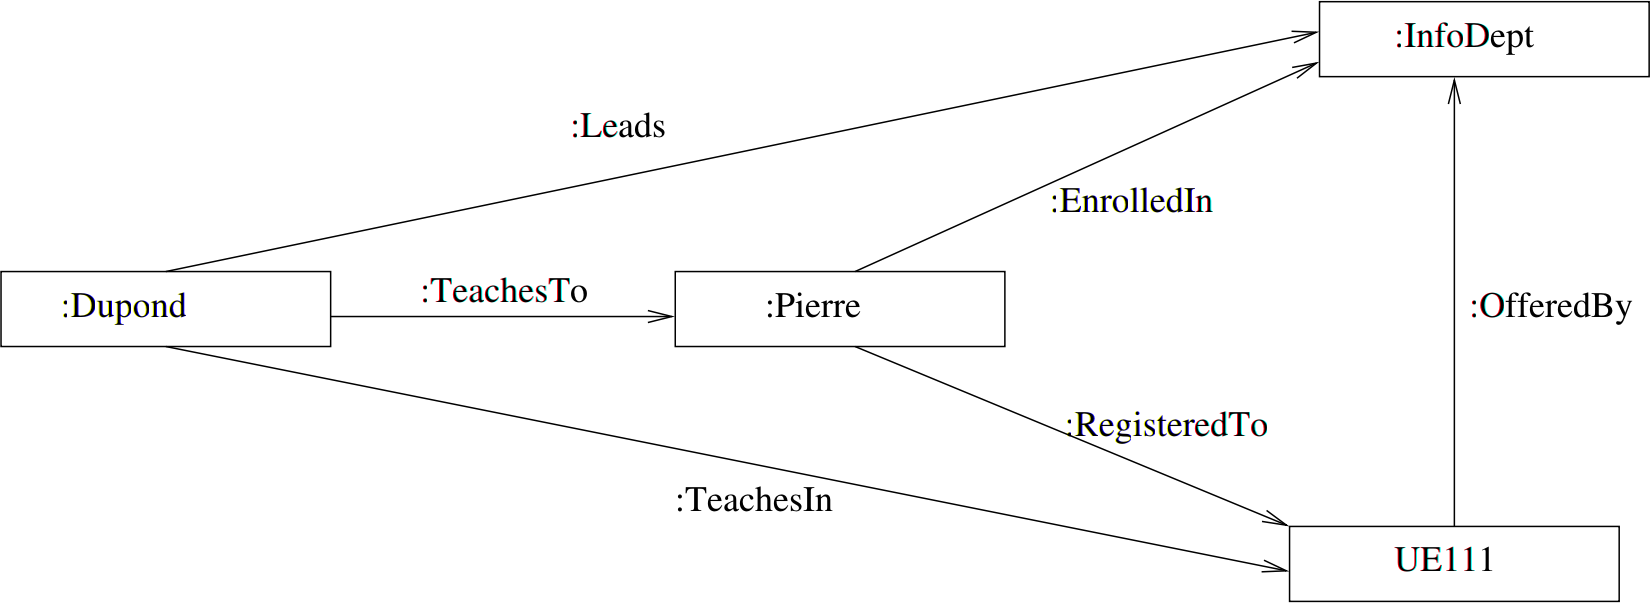
\includegraphics[width=11cm]{graph.png}
  \end{center}

  \triple{:Dupond :Leads :InfoDept} \\
  \triple{:Dupond :TeachesIn :UE111} \\
  \triple{:Dupond :TeachesTo :Pierre} \\
  \triple{:Pierre :EnrolledIn :InfoDept} \\
  \triple{:Pierre :RegisteredTo :UE111} \\
  \triple{:UE110 :OfferedBy :InfoDept}
\end{frame}

\begin{frame}
  \frametitle{RDF}
  \framesubtitle{Syntax}

  There are many different syntaxes for writing RDF triples, including:

  \pause

  \begin{itemize}
    \item XML (as used in \atweb),

    \pause

    \item Turtle,
    \item N-Triples,
    \item N-Quads,
    \item etc.
  \end{itemize}

  \pause

  However, we're going to focus on the abstract \triple{subject, predicate,
  object} syntax during this presentation.
\end{frame}

\begin{frame}
  \frametitle{RDFS}

  The \textit{schema language} for RDF. Allows specifying constraints on
  individuals and relationships used in RDF.

  \pause

  \medskip

  Some examples of these constraints are:

  \pause

  \begin{itemize}
    \item \texttt{rdf:type} (used to specify class membership of an individual),
    \item \texttt{rdfs:subClassOf} (subclass relationship between classes),
    \item \texttt{rdfs:subPropertyOf} (subproperty relationship between
      properties),
    \item \texttt{rdfs:domain} (domain of a property),
    \item \texttt{rdfs:range} (range of a property),
    \item etc.
  \end{itemize}
\end{frame}

\begin{frame}
  \frametitle{RDFS}
  \framesubtitle{\texttt{rdf:type}}

  Used to specify class membership.

  \pause

  \bigskip

  Syntax: \triple{i rdf:type C}.

  \pause

  \medskip

  First-order logic translation: $C(i)$.

  \pause

  \bigskip

  Examples:

  \begin{itemize}
    \item \triple{:Dupond rdf:type :AcademicStaff}
    \item \triple{:Pierre rdf:type :MasterStudent}
  \end{itemize}
\end{frame}

\begin{frame}
  \frametitle{RDFS}
  \framesubtitle{\texttt{rdfs:subClassOf}}

  Used to specify subclass relationships between classes.

  \pause

  \bigskip

  Syntax: \triple{C rdfs:subClassOf D}.

  \pause

  \medskip

  First-order logic translation: $\forall X (C(X) \implies D(X))$.

  \pause

  \bigskip

  Example:

  \begin{itemize}
    \item \triple{:MasterStudent rdfs:subClassOf :Student}
  \end{itemize}

  \pause

  Usage example:

  \begin{itemize}
    \item \triple{:Pierre rdf:type :MasterStudent}
  \end{itemize}

  \pause

  Which implies:

  \begin{itemize}
    \item \triple{:Pierre rdf:type :Student}
  \end{itemize}
\end{frame}

\begin{frame}
  \frametitle{RDFS}
  \framesubtitle{\texttt{rdfs:subPropertyOf}}

  Used to specify subproperty relationships between properties.

  \pause

  \bigskip

  Syntax: \triple{P rdfs:subPropertyOf R}.

  \pause

  \medskip

  First-order logic translation: $\forall X \forall Y (P(X, Y) \implies
                                                       R(X, Y))$.

  \pause

  \bigskip

  Example:

  \begin{itemize}
    \item \triple{:LateRegisteredTo rdfs:subPropertyOf :RegisteredTo}
  \end{itemize}

  \pause

  Usage example:

  \begin{itemize}
    \item \triple{:Alice :LateRegisteredTo :UE111}
  \end{itemize}

  \pause

  Which implies:

  \begin{itemize}
    \item \triple{:Alice :RegisteredTo :UE111}
  \end{itemize}
\end{frame}

\begin{frame}
  \frametitle{RDFS}
  \framesubtitle{\texttt{rdfs:domain}}

  Used to specify the domain of a property.

  \pause

  \bigskip

  Syntax: \triple{P rdfs:domain C}.

  \pause

  \medskip

  First-order logic translation: $\forall X \forall Y (P(X, Y) \implies C(X))$.

  \pause

  \bigskip

  Example:

  \begin{itemize}
    \item \triple{:TeachesTo rdfs:domain :AcademicStaff}
  \end{itemize}

  \pause

  Usage example:

  \begin{itemize}
    \item \triple{:Dupond :TeachesTo :Pierre}
  \end{itemize}

  \pause

  Which implies:

  \begin{itemize}
    \item \triple{:Dupond rdf:type :AcademicStaff}
  \end{itemize}
\end{frame}

\begin{frame}
  \frametitle{RDFS}
  \framesubtitle{\texttt{rdfs:range}}

  Used to specify the range of a property.

  \pause

  \bigskip

  Syntax: \triple{P rdfs:range D}.

  \pause

  \medskip

  First-order logic translation: $\forall X \forall Y (P(X, Y) \implies D(Y))$.

  \pause

  \bigskip

  Example:

  \begin{itemize}
    \item \triple{:TeachesTo rdfs:range :Student}
  \end{itemize}

  \pause

  Usage example:

  \begin{itemize}
    \item \triple{:Dupond :TeachesTo :Pierre}
  \end{itemize}

  \pause

  Which implies:

  \begin{itemize}
    \item \triple{:Pierre rdf:type :Student}
  \end{itemize}
\end{frame}

\begin{frame}
  \frametitle{OWL}

  The \textit{Web Ontology Language}. Extends RDFS with many additional
  constraints.

  \pause

  \medskip

  Some examples of such constraints:

  \pause

  \begin{itemize}
    \item \texttt{owl:disjointWith} (specifies class disjointness),
    \item \texttt{owl:unionOf} (defines a class as a union of other classes),
    \item \texttt{owl:intersectionOf} (defines a class as an intersection of
      other classes),
    \item \texttt{owl:minCardinality} (minimum cardinality of a relationship),
    \item \texttt{owl:maxCardinality} (maximum cardinality of a relationship),
    \item \texttt{owl:functionalProperty} (a property describes a mathematical function),
    \item \texttt{owl:symmetricProperty} ($R(X, Y)$ implies $R(Y, X)$),
    \item etc.
  \end{itemize}
\end{frame}

\begin{frame}
  \frametitle{SKOS}

  Stands for \textit{Simple Knowledge Organization System}. It allows
  structuring a vocabulary in a machine readable way.

  \pause

  \medskip

  It's a common data model for knowledge organization systems such as thesauri,
  classification schemes, subject heading systems and taxonomies. Typical uses
  include organizing large collections of objects such as books or museum
  artifacts.

  \pause

  \medskip

  SKOS is not for formal ontologies. It's not meant to express formal axioms
  nor allowing automatic reasoning. Instead, it's meant to be a \textit{simple}
  model with softer semantics that focuses on terminological information.

  \pause

  \medskip

  Used in \atweb to bridge the gap between data in scientific documents and the
  associated domain ontology.
\end{frame}

\begin{frame}
  \frametitle{SKOS}
  \framesubtitle{A sample SKOS graph}

  \begin{center}
    % Taken from http://dcevents.dublincore.org/IntConf/dc-2011/paper/view/69/36
    % Page 34
    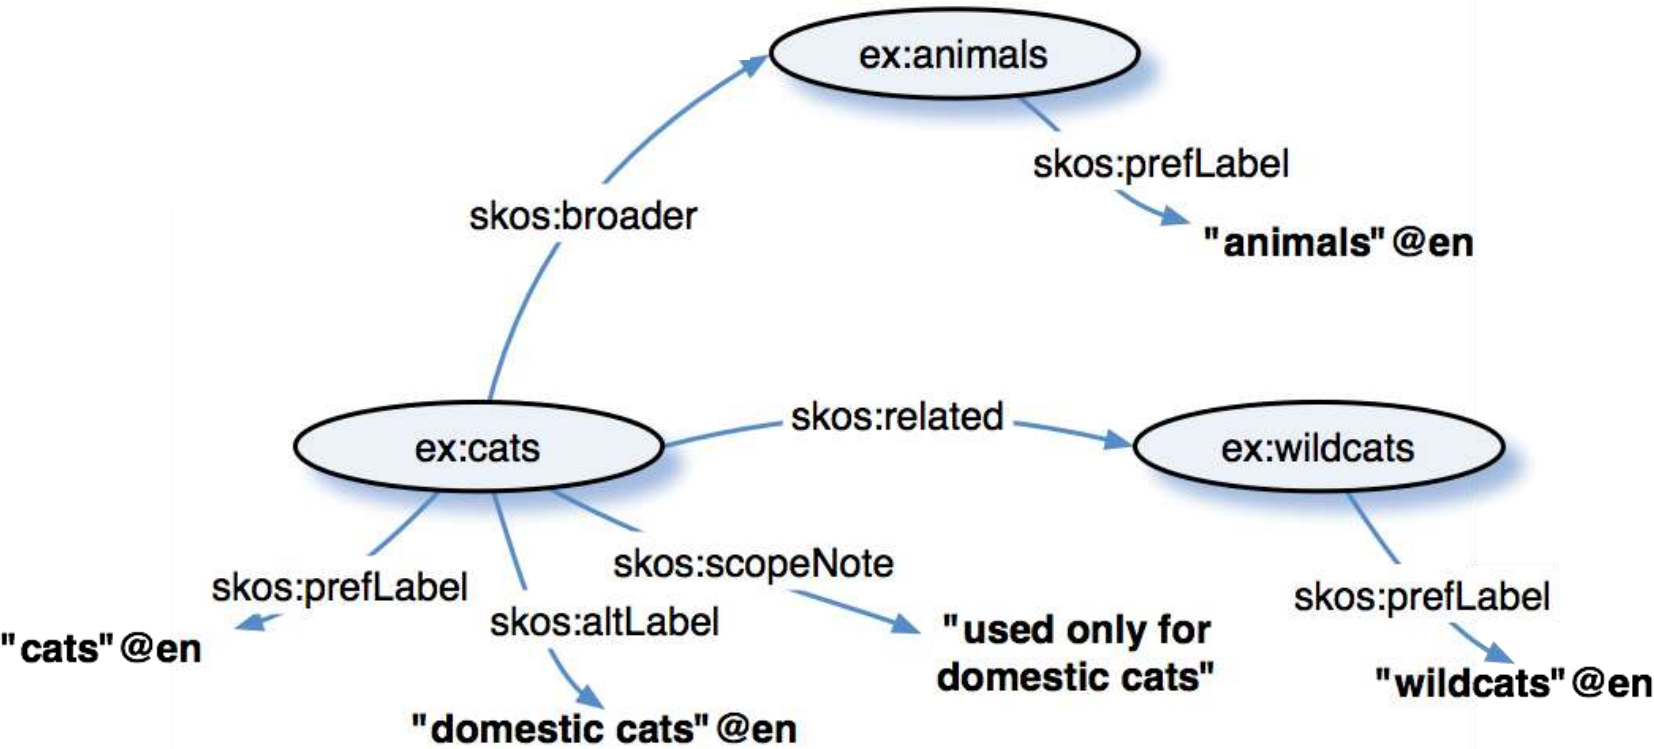
\includegraphics[width=11cm]{skos.png}
  \end{center}
\end{frame}

\begin{frame}
  \frametitle{SKOS}
  \framesubtitle{How it's used in \atweb}

  \begin{center}
    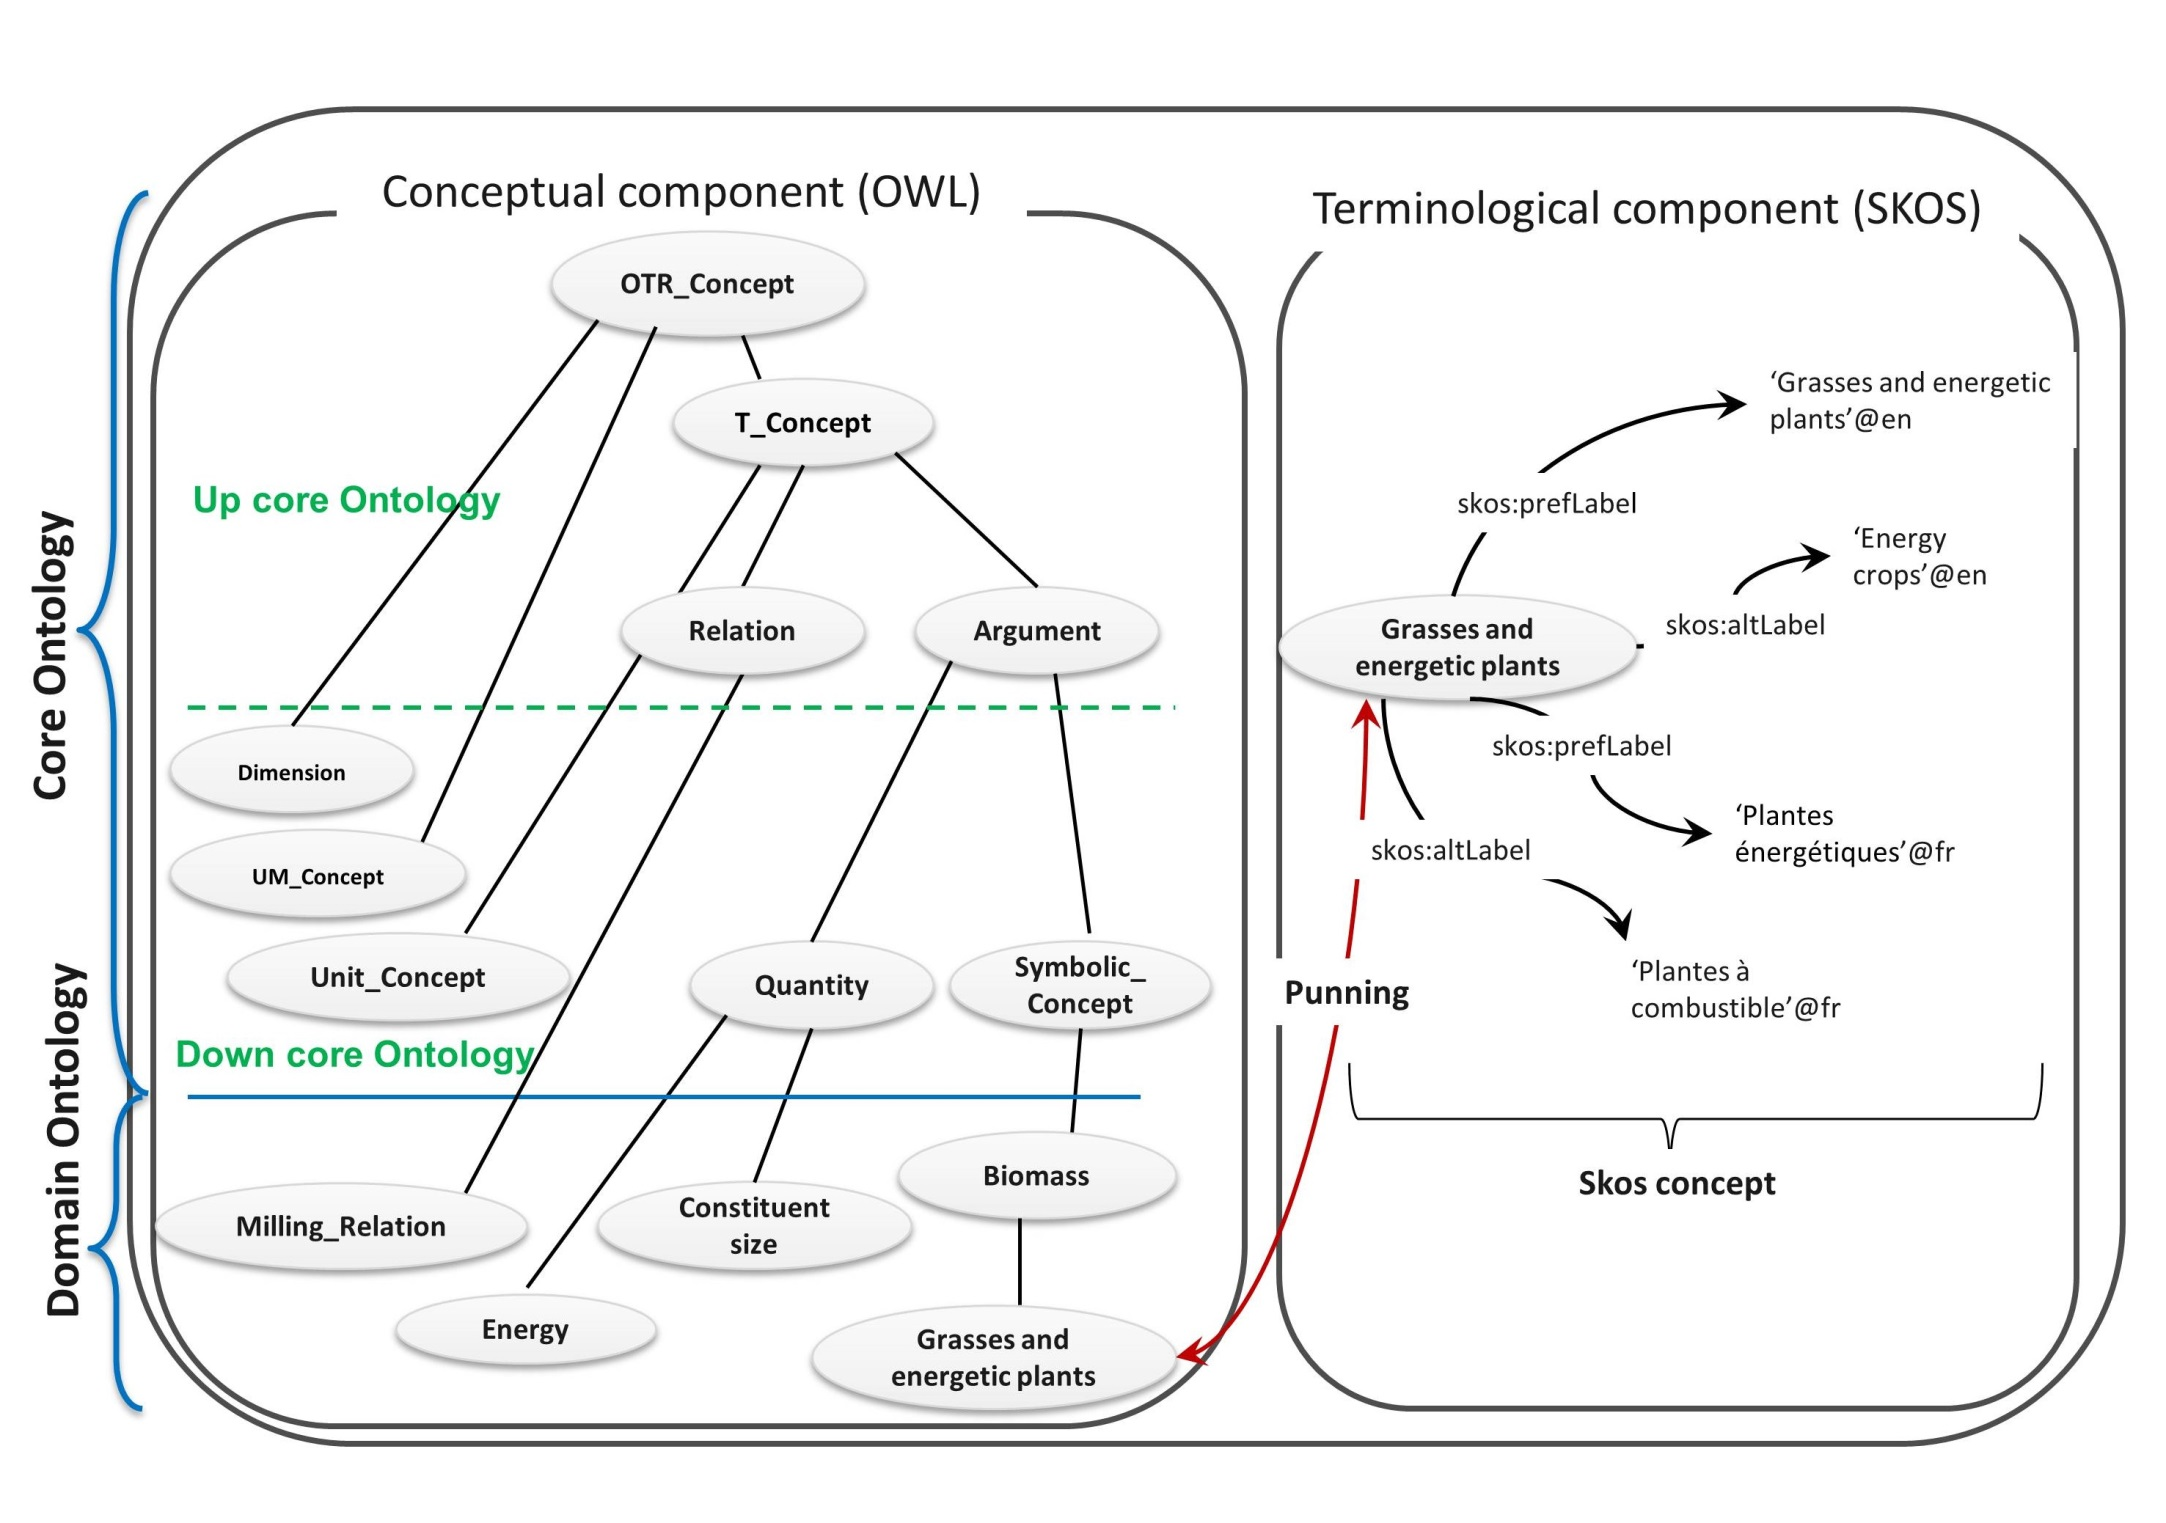
\includegraphics[width=11cm]{termino-ontological-resource.jpg}
  \end{center}
\end{frame}

\begin{frame}[fragile]
  \frametitle{SKOS}
  \framesubtitle{A SKOS concept taken from the biorefinery application}

  \begin{Verbatim}[fontsize=\scriptsize]
<skos:Concept rdf:ID="treated_corn_stover">
  <rdfs:subClassOf>
    <skos:Concept rdf:ID="corn_stover">
      <rdfs:subClassOf>
        <skos:Concept rdf:ID="grasses_and_energetic_plants">
          <rdfs:subClassOf rdf:resource="#biomass"/>
          <skos:prefLabel xml:lang="en">Grasses and energetic plants</skos:prefLabel>
          <skos:prefLabel xml:lang="fr">Herbes et plantes énergétiques</skos:prefLabel>
          <rdf:type rdf:resource="http://www.w3.org/2002/07/owl#Class"/>
        </skos:Concept>
      </rdfs:subClassOf>
      <skos:altLabel xml:lang="en">Maize stover</skos:altLabel>
      <skos:prefLabel xml:lang="en">Corn stover</skos:prefLabel>
      <skos:prefLabel xml:lang="fr">Fourrage de maïs</skos:prefLabel>
      <rdf:type rdf:resource="http://www.w3.org/2002/07/owl#Class"/>
    </skos:Concept>
  </rdfs:subClassOf>
  <skos:prefLabel xml:lang="en">Treated Corn stover</skos:prefLabel>
  <skos:prefLabel xml:lang="fr">Fourrage de maïs traité</skos:prefLabel>
  <rdf:type rdf:resource="http://www.w3.org/2002/07/owl#Class"/>
</skos:Concept>
  \end{Verbatim}
\end{frame}

\begin{frame}
  \frametitle{The n-ary relationship pattern used in \atweb}
  \framesubtitle{Motivation}

  \begin{itemize}
    \item RDF relations are binary (they only involve a subject and an object.)

    \pause

    \item Experimental data often involve more than two individuals:

    \pause

    \begin{itemize}
      \item input flow,
      \item control parameters,
      \item output flow
    \end{itemize}

    \pause

    \item There are many ways to represent n-ary relations using RDF triples.

    \pause

    \item \textbf{Proposed solution:} create an n-ary relationship design
      pattern specifically taylored to model experimental data.
  \end{itemize}
\end{frame}

\begin{frame}
  \frametitle{The n-ary relationship pattern used in \atweb}
  \framesubtitle{An ontology for n-ary relationships}

  \begin{center}
    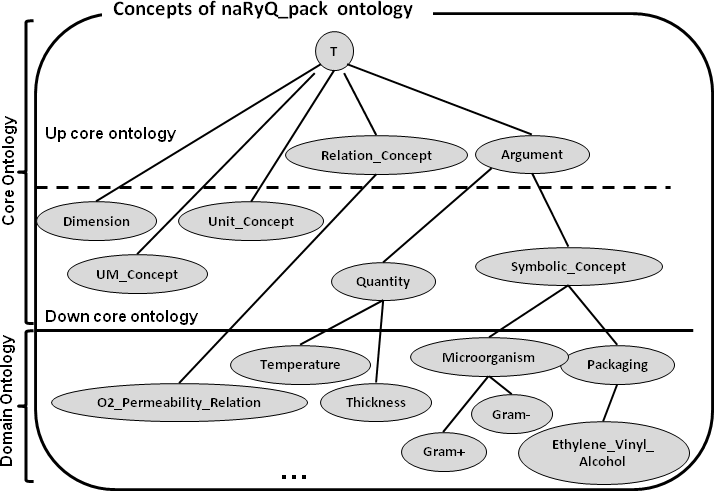
\includegraphics[width=10cm]{ontology.png}
  \end{center}
\end{frame}

\begin{frame}[fragile]
  \frametitle{The n-ary relationship pattern used in \atweb}
  \framesubtitle{An ontology for n-ary relationships: OWL definition}

  \begin{Verbatim}[fontsize=\tiny]
<!-- Core ontology -->
<owl:Class rdf:ID="Relation_Concept">
<owl:Class rdf:ID="Argument"/>
<owl:Class rdf:ID="Quantity">
  <rdfs:subClassOf rdf:resource="#Argument"/>
</owl:Class>
<owl:Class rdf:ID="Symbolic_Concept">
  <rdfs:subClassOf rdf:resource="#Argument"/>
</owl:Class>
...

<!-- Domain ontology -->
<owl:Class rdf:ID="O2Permeability">
  <rdfs:subClassOf rdf:resource="#Quantity"/>
</owl:Class>
<owl:Class rdf:ID="Packaging">
  <rdfs:subClassOf rdf:resource="#Symbolic_Concept"/>
</owl:Class>
<rdf:ObjectProperty rdf:ID="hasO2Permeability">
    <rdfs:domain rdf:resource="#Relation_Concept"/>
    <rdfs:range rdf:resource="#O2Permeability"/>
</rdf:ObjectProperty>
<rdf:ObjectProperty rdf:ID="hasPackaging">
    <rdfs:domain rdf:resource="#Relation_Concept"/>
    <rdfs:range rdf:resource="#Packaging"/>
</rdf:ObjectProperty>
...
  \end{Verbatim}
\end{frame}

\begin{frame}
  \frametitle{The n-ary relationship pattern used in \atweb}
  \framesubtitle{Some observations}

  \begin{itemize}
    \item This design requires experiments to have \textit{at least} two
      input/control parameters.

    \pause

    \item It allows optional and mandatory parameters.

    \pause

    \item The order of the input parameters doesn't matter.

    \pause

    \item Each instance of an n-ary relation has \textit{exactly} one output.
  \end{itemize}
\end{frame}

\begin{frame}
  \frametitle{A sample n-ary relationship}

  \begin{center}
    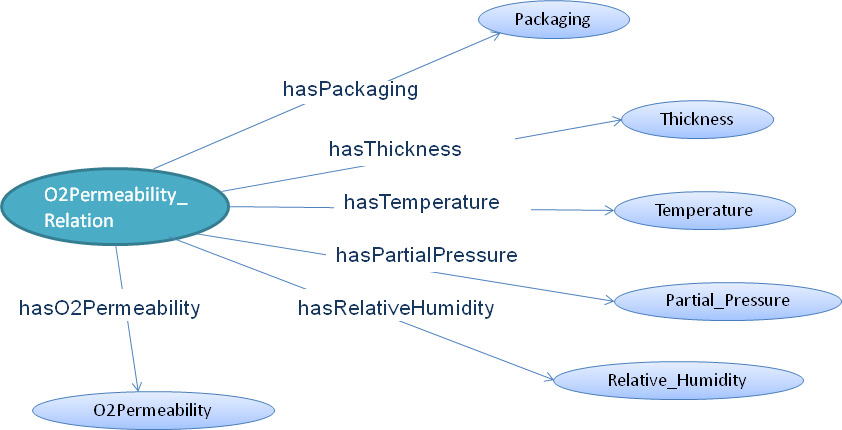
\includegraphics[width=11cm]{relation.png}
  \end{center}
\end{frame}

\begin{frame}[fragile]
  \frametitle{A sample n-ary relationship}
  \framesubtitle{OWL definition (I)}

  \begin{Verbatim}[fontsize=\scriptsize]
<owl:Class rdf:ID="O2Permeability_Relation">
  <rdfs:subClassOf rdf:resource="#Relation"/>

  <rdfs:subClassOf>
    <owl:Restriction>
      <owl:onProperty rdf:resource="#hasO2Permeability"/>
      <owl:allValuesFrom rdf:resource="#O2Permeability"/>
    </owl:Restriction>
  </rdfs:subClassOf>

  <rdfs:subClassOf>
    <owl:Restriction>
      <owl:onProperty rdf:resource="#hasO2Permeability"/>
      <owl:cardinality rdf:datatype="&xsd;nonNegativeInteger">
        1
      </owl:cardinality>
    </owl:Restriction>
  </rdfs:subClassOf>
  \end{Verbatim}
\end{frame}

\begin{frame}[fragile]
  \frametitle{A sample n-ary relationship}
  \framesubtitle{OWL definition (II)}

  \begin{Verbatim}[fontsize=\scriptsize]
  <rdfs:subClassOf>
    <owl:Restriction>
      <owl:onProperty rdf:resource="#hasPackaging"/>
      <owl:allValuesFrom rdf:resource="#Packaging"/>
    </owl:Restriction>
  </rdfs:subClassOf>

  <rdfs:subClassOf>
    <owl:Restriction>
      <owl:onProperty rdf:resource="#hasPackaging"/>
      <owl:mincardinality rdf:datatype="&xsd;nonNegativeInteger">
        1
      </owl:cardinality>
    </owl:Restriction>
  </rdfs:subClassOf>

  <rdfs:subClassOf>
    <owl:Restriction>
      <owl:onProperty rdf:resource="#hasThickness"/>
      <owl:allValuesFrom rdf:resource="#Thickness"/>
    </owl:Restriction>
  </rdfs:subClassOf>
  \end{Verbatim}
\end{frame}

\begin{frame}[fragile]
  \frametitle{A sample n-ary relationship}
  \framesubtitle{OWL definition (III)}

  \begin{Verbatim}[fontsize=\scriptsize]
  <rdfs:subClassOf>
    <owl:Restriction>
      <owl:onProperty rdf:resource="#hasTemperature"/>
      <owl:allValuesFrom rdf:resource="#Temperature"/>
    </owl:Restriction>
  </rdfs:subClassOf>

  <rdfs:subClassOf>
    <owl:Restriction>
      <owl:onProperty rdf:resource="#hasPartialPressure"/>
      <owl:allValuesFrom rdf:resource="#Partial_Pressure"/>
    </owl:Restriction>
  </rdfs:subClassOf>

  <rdfs:subClassOf>
    <owl:Restriction>
      <owl:onProperty rdf:resource="#hasRelativeHumidity"/>
      <owl:allValuesFrom rdf:resource="#Relative_Humidity"/>
   </owl:Restriction>
  </rdfs:subClassOf>
</owl:Class>
  \end{Verbatim}
\end{frame}

\begin{frame}
  \frametitle{Example of an annotated scientific document}
  \framesubtitle{Table extracted using the \atweb platform}

  \begin{center}
    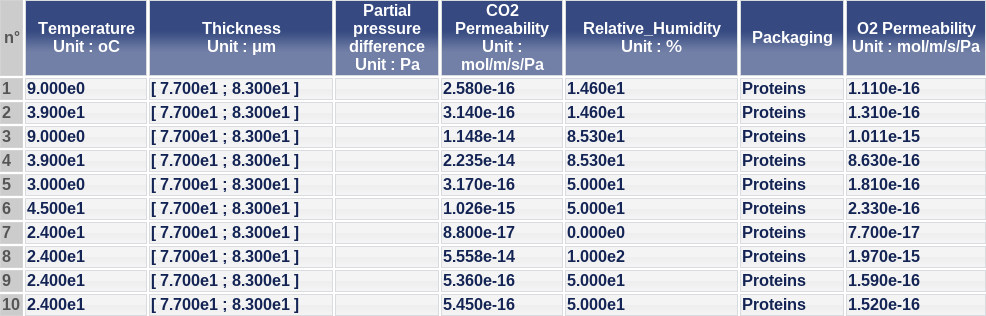
\includegraphics[width=10cm]{table.png}
  \end{center}
\end{frame}

\begin{frame}[fragile]
  \frametitle{Example of an annotated scientific document}
  \framesubtitle{RDF annotations (I)}

  \begin{Verbatim}[fontsize=\tiny]
<onto:hasTable>
  <onto:Table rdf:about="Table_160">
    <onto:hasForRow>
      <onto:Row rdf:about="Row-5_160">
        <onto:hasForRelation>

          <!-- O2 permeability relation instance -->
          <domain:o2_permeability_relation rdf:about="o2_permeability_relation_Row-5_160">
            <onto:hasForDegree rdf:datatype="http://www.w3.org/2001/XMLSchema#double"
            >1.0</onto:hasForDegree>

            ...
  \end{Verbatim}
\end{frame}

\begin{frame}[fragile]
  \frametitle{Example of an annotated scientific document}
  \framesubtitle{RDF annotations (II)}

  \begin{Verbatim}[fontsize=\tiny]
            <!-- Experiment output -->
            <core:hasResultConcept>
              <onto:Cell rdf:about="Cell-6_Row-5_160">
                <rdf:type rdf:resource="/resources/hSC9z#o2_permeability"/>
                <onto:hasForOriginalValue rdf:datatype="http://www.w3.org/2001/XMLSchema#string"
                >233</onto:hasForOriginalValue>
                <onto:hasForColumnNumber rdf:datatype="http://www.w3.org/2001/XMLSchema#integer"
                >6</onto:hasForColumnNumber>
                <onto:hasForFS>
                  <onto:CFS rdf:about="CFS_Cell-6_Row-5_160">
                    <rdf:type rdf:resource="/resources/atWeb/annotation/Scalar"/>
                    <onto:hasForUnit rdf:resource="/resources/hSC9z#Mole_Per_Meter_Per_Second_Per_Pascal"/>
                    <onto:hasForFuzzyElement>
                      <onto:FuzzySet rdf:about="FS_Cell-6_Row-5_160">
                        <onto:hasForMaxKernel rdf:datatype=
                        "http://www.w3.org/2001/XMLSchema#string"
                        >2.330e-16</onto:hasForMaxKernel>
                        <onto:hasForMinKernel rdf:datatype=
                            "http://www.w3.org/2001/XMLSchema#string"
                            >2.330e-16</onto:hasForMinKernel>
                            <onto:hasForMinSupport rdf:datatype=
                            "http://www.w3.org/2001/XMLSchema#string"
                            >2.330e-16</onto:hasForMinSupport>
                            <onto:hasForMaxSupport rdf:datatype=
                            "http://www.w3.org/2001/XMLSchema#string"
                            >2.330e-16</onto:hasForMaxSupport>
                      </onto:FuzzySet>
                    </onto:hasForFuzzyElement>
                  </onto:CFS>
                </onto:hasForFS>
              </onto:Cell>
            </core:hasResultConcept>
  \end{Verbatim}
\end{frame}

\begin{frame}[fragile]
  \frametitle{Example of an annotated scientific document}
  \framesubtitle{RDF annotations (III)}

  \begin{Verbatim}[fontsize=\tiny]
            <!-- Experiment input parameter: temperature -->
            <core:hasAccessConcept>
              <onto:Cell rdf:about="Cell-0_Row-5_160">
                <rdf:type rdf:resource="/resources/hSC9z#temperature"/>
                <onto:hasForOriginalValue rdf:datatype="http://www.w3.org/2001/XMLSchema#string"
                >45</onto:hasForOriginalValue>
                <onto:hasForColumnNumber rdf:datatype="http://www.w3.org/2001/XMLSchema#integer"
                >0</onto:hasForColumnNumber>
                <onto:hasForFS>
                  <onto:CFS rdf:about="CFS_Cell-0_Row-5_160">
                    <rdf:type rdf:resource="/resources/atWeb/annotation/Scalar"/>
                    <onto:hasForUnit rdf:resource="/resources/hSC9z#Degree_Celsius"/>
                    <onto:hasForFuzzyElement>
                      <onto:FuzzySet rdf:about="FS_Cell-0_Row-5_160">
                        <onto:hasForMaxKernel rdf:datatype=
                        "http://www.w3.org/2001/XMLSchema#string"
                        >4.500e1</onto:hasForMaxKernel>
                        <onto:hasForMinKernel rdf:datatype=
                        "http://www.w3.org/2001/XMLSchema#string"
                        >4.500e1</onto:hasForMinKernel>
                        <onto:hasForMinSupport rdf:datatype=
                        "http://www.w3.org/2001/XMLSchema#string"
                        >4.500e1</onto:hasForMinSupport>
                        <onto:hasForMaxSupport rdf:datatype=
                        "http://www.w3.org/2001/XMLSchema#string"
                        >4.500e1</onto:hasForMaxSupport>
                      </onto:FuzzySet>
                    </onto:hasForFuzzyElement>
                  </onto:CFS>
                </onto:hasForFS>
              </onto:Cell>
            </core:hasAccessConcept>
  \end{Verbatim}
\end{frame}

\begin{frame}[fragile]
  \frametitle{Example of an annotated scientific document}
  \framesubtitle{RDF annotations (IV)}

  \begin{Verbatim}[fontsize=\tiny]
            <!-- Experiment input parameter: thickness -->
            <core:hasAccessConcept>
              <onto:Cell rdf:about="Cell-1_Row-5_160">
                <rdf:type rdf:resource="/resources/hSC9z#thickness"/>
                <onto:hasForOriginalValue rdf:datatype="http://www.w3.org/2001/XMLSchema#string"
                ></onto:hasForOriginalValue>
                <onto:hasForColumnNumber rdf:datatype="http://www.w3.org/2001/XMLSchema#integer"
                >1</onto:hasForColumnNumber>
                <onto:hasForFS>
                  <onto:CFS rdf:about="CFS_Cell-1_Row-5_160">
                    <rdf:type rdf:resource="/resources/atWeb/annotation/Interval"/>
                    <onto:hasForUnit rdf:resource="/resources/hSC9z#Micrometer"/>
                    <onto:hasForFuzzyElement>
                      <onto:FuzzySet rdf:about="FS_Cell-1_Row-5_160">
                        <onto:hasForMaxKernel rdf:datatype=
                        "http://www.w3.org/2001/XMLSchema#string"
                        >8.300e1</onto:hasForMaxKernel>
                        <onto:hasForMinKernel rdf:datatype=
                        "http://www.w3.org/2001/XMLSchema#string"
                        >7.700e1</onto:hasForMinKernel>
                        <onto:hasForMinSupport rdf:datatype=
                        "http://www.w3.org/2001/XMLSchema#string"
                        >7.700e1</onto:hasForMinSupport>
                        <onto:hasForMaxSupport rdf:datatype=
                        "http://www.w3.org/2001/XMLSchema#string"
                        >8.300e1</onto:hasForMaxSupport>
                      </onto:FuzzySet>
                    </onto:hasForFuzzyElement>
                  </onto:CFS>
                </onto:hasForFS>
              </onto:Cell>
            </core:hasAccessConcept>
  \end{Verbatim}
\end{frame}

\begin{frame}[fragile]
  \frametitle{Example of an annotated scientific document}
  \framesubtitle{RDF annotations (V)}

  \begin{Verbatim}[fontsize=\tiny]
            ...
            <core:hasAccessConcept rdf:resource="Cell-2_Row-5_160"/>
            <core:hasAccessConcept rdf:resource="Cell-4_Row-5_160"/>
            <core:hasAccessConcept rdf:resource="Cell-5_Row-5_160"/>
          </domain:o2_permeability_relation>
        </onto:hasForRelation>
        ...
  \end{Verbatim}
\end{frame}

\begin{frame}[fragile]
  \frametitle{Example of an annotated scientific document}
  \framesubtitle{RDF annotations (VI)}

  \begin{Verbatim}[fontsize=\tiny]
        <!-- Cell "Relative Humidity (%)" -->
        <onto:hasForCell>
          <onto:Cell rdf:about="Cell-4_Row-5_160">
            <rdf:type rdf:resource="/resources/hSC9z#relative_humidity"/>
            <onto:hasForOriginalValue rdf:datatype="http://www.w3.org/2001/XMLSchema#string"
            >50</onto:hasForOriginalValue>
            <onto:hasForColumnNumber rdf:datatype="http://www.w3.org/2001/XMLSchema#integer"
            >4</onto:hasForColumnNumber>
            <onto:hasForFS>
              <onto:CFS rdf:about="CFS_Cell-4_Row-5_160">
                <rdf:type rdf:resource="/resources/atWeb/annotation/Scalar"/>
                <onto:hasForUnit rdf:resource="/resources/hSC9z#Percent"/>
                <onto:hasForFuzzyElement>
                  <onto:FuzzySet rdf:about="FS_Cell-4_Row-5_160">
                    <onto:hasForMaxKernel rdf:datatype="http://www.w3.org/2001/XMLSchema#string"
                    >5.000e1</onto:hasForMaxKernel>
                    <onto:hasForMinKernel rdf:datatype="http://www.w3.org/2001/XMLSchema#string"
                    >5.000e1</onto:hasForMinKernel>
                    <onto:hasForMinSupport rdf:datatype="http://www.w3.org/2001/XMLSchema#string"
                    >5.000e1</onto:hasForMinSupport>
                    <onto:hasForMaxSupport rdf:datatype="http://www.w3.org/2001/XMLSchema#string"
                    >5.000e1</onto:hasForMaxSupport>
                  </onto:FuzzySet>
                </onto:hasForFuzzyElement>
              </onto:CFS>
            </onto:hasForFS>
          </onto:Cell>
        </onto:hasForCell>
  \end{Verbatim}
\end{frame}

\begin{frame}[fragile]
  \frametitle{Example of an annotated scientific document}
  \framesubtitle{RDF annotations (VII)}

  \begin{Verbatim}[fontsize=\tiny]
        <!-- Cell "Packaging" -->
        <onto:hasForCell>
          <onto:Cell rdf:about="Cell-5_Row-5_160">
            <rdf:type rdf:resource="/resources/hSC9z#packaging"/>
            <onto:hasForOriginalValue rdf:datatype="http://www.w3.org/2001/XMLSchema#string"
            >Wheat gluten</onto:hasForOriginalValue>
            <onto:hasForColumnNumber rdf:datatype="http://www.w3.org/2001/XMLSchema#integer"
            >5</onto:hasForColumnNumber>
            <onto:hasForFS>
              <onto:DFS rdf:about="DFS_Cell-5_Row-5_160">
                <onto:hasForElement>
                  <domain:proteins rdf:about="proteins_Cell-5_Row-5_160">
                    <onto:hasForDegree rdf:datatype="http://www.w3.org/2001/XMLSchema#double"
                    >1.0</onto:hasForDegree>
                  </domain:proteins>
                </onto:hasForElement>
              </onto:DFS>
            </onto:hasForFS>
          </onto:Cell>
        </onto:hasForCell>

        <!-- More cells -->
        ...
      </onto:Row>
    </onto:hasForRow>

    <!-- More rows -->
    ...
  </onto:Table>
</onto:hasTable>
  \end{Verbatim}
\end{frame}

\begin{frame}
  \begin{center}
    \Huge{Thanks!}
  \end{center}
\end{frame}

\end{document}
